\section{Prestudy}
\label{sec:prestudy}
%Intro - what the prestudy was
In order to inform the development of the project, and provide a reasonable basis for some of the design decisions made about the system, an initial prestudy was run with questions covering a wide range of relevant areas.
%Justifications - some detail about contents
The primary intention of the survey was to find out how people currently consume TV programmes and related streaming media, and their responses to the adverts that support the services they use.
There were questions on format and frequency of media consumption, and typical actions during advertisement presentation.
The study also included questions about individual levels of acceptance of the use of personal information for advertisement targeting, and an opportunity to share further personal opinions and comments in an optional free text question.
%Conclusion - the prestudy was useful
Ultimately, the wide coverage of questions gave many useful insights into existing viewer habits and responses.

%Intro - what the data was for
The main use of the data collected during the survey was to support and justify system development decisions throughout the course of the project. 
%Justification - specific hopes for the results
The questions were written to elicit information from the participants in support of several specific purposes, in addition to the basic background information about existing viewing habits.
One intended function of the results was to establish which features of an advert had the most influence on user attention -- this would allow development to be focused upon the best techniques to retain user attention to adverts, thereby making the product a more desirable option for advertisers, and resulting in greater profits for advertisers and greater satisfaction for users.
Another intended outcome was to discover whether typical advertisement responses provided scope for alternative attention retention techniques; for example, if users typically refocused their activities onto other devices during advertisement breaks, the provision of audio-only advertisements could provide an avenue for successful impressions despite loss of visual attention.
%Conclusion - the data was relevant
Determining how users respond to existing adverts in existing systems was an important prerequisite to tailoring development work so that the system is as effective as possible, and the survey questions were designed to support that aim.


% Purpose of the study:\\
% Collect data on how people consume media and adverts\\
% Inform the development of features for the project\\
% Elicit basic information about viewer habits

\subsection{Methodology}

% The prestudy was performed early in the project --- 10/20/2012 --- to allow the results to be considered into the design of your4.tv. The study was hosted as a short questionnaire online at the url \url{www.http://your4.tv/#prestudy}, designed to be easy and quick to fill out to maximise responses, with each entry automatically entered into a spreadsheet upon submission. At the time of writing, the prestudy is still available online, and a listing of the prestudy questions can be found in Appendix~\ref{sec:appendix_prestudy_questions}.

% The url was shared amongst a demographic of students, the target audience of the system, where each submission was anonymous, and run for 7 days gathering 67 responses before the results were analysed.

% The prestudy page as presented to participants is available at \href{http://your4.tv/\#prestudy}{\texttt{your4.tv/\#prestudy}} 

%Intro - we wanted efficiency
To help ensure that the prestudy results were relevant and informative, close attention was paid to certain aspects of the study methodology.
%Justification - this was how we got it
%-Selected students as a sample - representative (find reference)\\
\citet{viacom} reports that young people (the 18-24 demographic) watch TV on tablets more than any other demographic, and so the prestudy was directed largely towards this group. %TODO Maybe mention Project4's target audience, and available adverts
%-Protected results, ethics number 4315\\
Following the guidelines of the governing body, the questionnaire draft was submitted to ERGO, and recieved ecthical approval to proceed (study number 4315).
%-Performed early\\
Since the survey outcomes were an important influencing factor in the continued development of the system, it was essential that the prestudy was completed early in the lifetime of the project. Once the intention and form of the questions had been finalised, the survey was created and publicised as widely as possible.
%Conclusion - aspects of how the survey was run made it more successful
By 

%Intro - we wanted lots of data
So that anomalous results did not unduly skew the outcome of the study, and to ensure broad coverage and increase the possible diversity of viewpoints captured, it was important to attempt to maximise the number of responses the survey would recieve.
%Justification - we did these things to induce people to answer
%We were also keen to ensure that as many people as possible would provide useful information
%-Short and easy and anonymous\\
One approach taken was to make the questionnaire as quick and painless as possible to complete
The survey design was intentionally short and minimal, to maximise the likelihood of agreement, we will also make it clear to any potential participant that no personally identifiable information will be collected and that they will not be contacted about their responses. %TODO: talk about using an URL
To perform this study an anonymous questionnaire has been chosen as the best approach.
This is because the information we gather will be used to tailor our service but will not require any further interaction on the part of the set of participants as they will not be provided with our product, only asked their opinion of existing and potential systems.

with each entry automatically entered into a spreadsheet upon submission.


%-Webpage\\
%-Spread via social networking sites\\
%Conclusion - This helped: we got a large number of results as discussed in the following section


%Note
The prestudy page as presented to participants is still available online\footnote{Your4 Prestudy Questionnaire -- \footurl{http://your4.tv/\#prestudy}} and a listing of the questions can be found in Appendix~\ref{sec:appendix_prestudy_questions}. 


\subsection{Survey outcome}



 - Analysis\\
  - Specific interest\\
  - Resulting decisions\\

Results:\\
67 student participants\\
Discovered specific features we should focus on:\\
Relevant adverts\\
Ability to skip adverts\\
... suggests that the product we propose will improve the ...

\subsubsection{Attention by media type}
%Question: How often do you pay attention to adverts served with the following media?
\begin{figure}[H]
	\vspace{-10pt}
	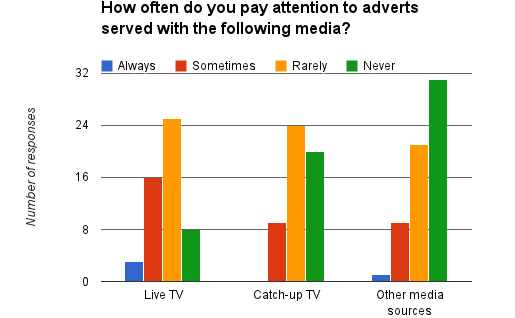
\includegraphics[width=\textwidth]{images/prestudy_media.png}
	\caption{User responses to the question ``How often do you pay attention to adverts served with the following media?''}
	\label{fig:prestudy_media}
	\vspace{-15pt}
\end{figure}
As can be seen in Figure~\ref{fig:prestudy_media}, only a small minority of participants reported to always pay attention adverts shown. In particular, amongst viewers watching other media such as Youtube, more than half of them never watch any of the advertisements at all - from the free text responses, it seem this is largely people using ad blocking programs. On the other hand, a far larger proportion of viewers `Always' or `Sometimes' watch adverts on live TV, which is certainly good news for a platform such as your4.tv.

\subsubsection{Advertisement responses}
%Question: If you do not pay attention to adverts, which of the following do you do instead? (multiple choice)
\begin{figure}[H]
	\vspace{-10pt}
	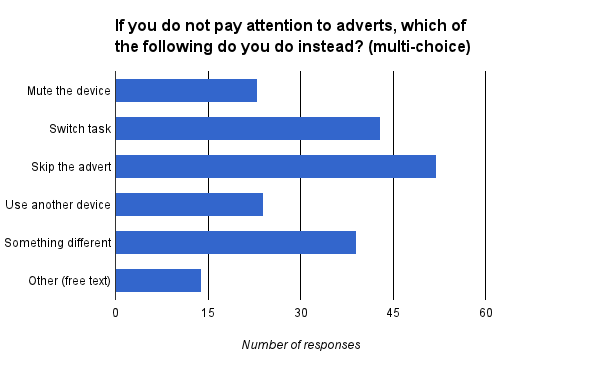
\includegraphics[width=\textwidth]{images/prestudy_alternatives.png}
	\caption{User responses to the question ``If you do not pay attention to adverts, which of the following do you do instead?''}
	\label{fig:prestudy_alternatives}
	\vspace{-15pt}
\end{figure}
Having seen that almost everyone ignores adverts sometimes, we also asked what people did instead of paying attention to them. Again, we can see that more than three quarters of the respondents skip adverts at least occasionally, where possible. We found that a few of the respondents mentioned `zoning out' and losing interest during ad breaks - we can also see that people use the advertisement time to do other tasks - generally on the same device, but less frequently on another one, or something completely different like making tea, etc. We use this data to help inform the development of functionality for the system.

\subsubsection{Influential Aspects}
%Question: How much do the following aspects influence how likely you are to watch an advert?
\begin{figure}[H]
	\vspace{-10pt}
	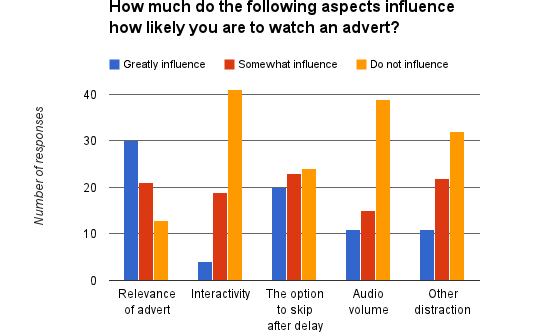
\includegraphics[width=\textwidth]{images/prestudy_influence.png}
	\caption{User responses to the question ``How much do the following aspects influence how likely you are to watch an advert?''}
	\label{fig:prestudy_influence}
	\vspace{-15pt}
\end{figure}
Finally, we looked at which specific aspects affected why people were likely to watch an advert (or not), with some interesting results. The two factors with the largest influence were the relevance of the advertisement and whether or not there was opportunity to skip it - both of which are addressed in the service we are developing. We also found, through analysing the free text responses, that people have a generally poor opinion of adverts that force a response from the user, whether they be obnoxiously loud, or simply require the user to interact with them before delivering content. Again, we can refer to these findings to help us to design a product that people will actually use. 
%TODO: do we mention the retrospecive need to define positive vs. negative influence?


